\chapter{Problematika vývoje rozšíření pro VS Code}

Jak už bylo zmíněno v úvodní kapitole, na oficiálním webu s rozšířeními pro VS Code \cite{marketplace} najdeme spousty aplikací, které vývojářům pomáhají např. s "debuggováním" kódu, analýzou dat, strojovým učením (machine learning), atd... Rozšíření pro Monkey C však nejsou zastoupena v tak hojném počtu, jako ostatní jazyky, což lze vidět v tabulce níže \ref{tab:statsTable}. V této kapitole budou popsány komponenty, které jsou stěžejní pro vytvoření překladače jazyka, parseru jazyka a následně rozšíření samotného.\\

\begin{table}
	\centering
	\caption{počet výsledků po vyhledání daného jazyka na marketplace \cite{marketplace}}
	\label{tab:statsTable}
	\begin{tabular}{lr}
			\toprule
			název jazyka & počet výsledků\\
			\midrule
			C Sharp & 169 \\
			Java & 2521 \\
			Python & 454 \\
			R & 6350 \\
			Monkey C & 2 \\
			\bottomrule
	\end{tabular}
\end{table}

\section{Visual Studio Code}
Visual Studio Code \cite{VSCODE_2020} je editor zdrojového kódu vytvořený společností Microsoft pro operační Windows, Linux a MacOS, který podporuje stovky druhů jazyků. Je naprogramován v jazycích JavaScript a Typescript a nabízí spoustu užitečných funkcí, mezi které patří podpora ladění kodu, zvýrazňování syntaxe, automatické doplňování a našeptávání kódu, odsazování textu, intuitivní klávesové zkratky, které usnadňují navigaci v kódu, atd… Cílem práce je integrovat většinu těchto funkcí a možností do finálního rozšíření.

\section{Typescript}
TypeScript \cite{TypeScript_wikipedia_2020} je open-source programovací jazyk vyvinutý společností Microsoft. Jedná se o nádstavbu nad jazykem JavaScript,
která jej rozšiřuje o statické typování a další atributy, které známe z objektově orientovaného programování jako jsou třídy, moduly a další. Samotný kód psaný v jazyce TypeScript se kompiluje do jazyka JavaScript. Jelikož je tento jazyk nádstavbou nad JavaScriptem, je každý JavaScript kód automaticky validním TypeScript kódem.\\
S programovacím jazykem Typescript jsem na začátku této práce mnohem menší zkušenosti, než např. s programovacími jazyky C Sharp nebo JavaScript. V průběhu studia jsem se však setkal s JavaScriptem při vývoji internetových aplikací. A jelikož je Typescript pouze nádstavba JavaScriptu a objektově orientované programování mě bylo dobře známé z jazyka C Sharp, nebylo obtížné se veškeré chybějící potřebné znalosti rychle doučit.

\section{Komponenty potřebné pro tvorbu rozšíření}
Předtím, než bude možné začít pracovat na samotném rozšíření, je potřeba obstarat několik důležitých nástrojů a komponent, jenž jsou klíčové při vývoji. Nejdůležitějším nástrojem pro vývoj rozšíření je však ANTLR, který je popsán v sekci \ref{antlr}.

\subsection{Gramatika}
Jako první je potřeba definovat popis jazyka Monkey C. V tomto případě je jazyk Monkey C popsán prostřednictvím bezkontextové gramatiky, která formálně definuje syntax (pravidla) jazyka. Jedná se, ve své podstatě, o soubor pravidel, kde každé pravidlo reprezentuje určitou strukturu či frázi jazyka. Z tohoto formálního popisu je ANTLR schopen vygenerovat parser daného jazyka, který dokáže automaticky sestavit datovou strukturu, která se nazývá buďto "parse tree" nebo "syntax tree", což v češtině znamená \textbf{syntaktický strom}. Tento syntaktický strom poté reprezentuje, jak přesně je gramatika schopna rozpoznávat vstupní data (např. fragment kódu).\\
Jelikož je v této práci použit ANTLR verze 4, je klíčové, aby název souboru obsahující gramatiku končil příponou .g4, v tomto případě soubor nese název \textbf{MonkeyC.g4}. 
\\
Na obrázku \ref{img:grammar} lze vidět prvních pár řádků Monkey C gramatiky. Gramatika obsahuje spoustu známých klíčových slov, nebo-li tokenů, např. "CLASS", "FUNCTION", "USING", atd...

\section{ANTLR - Nástroj pro generování překladače} \label{antlr}
ANTLR nebo také ANother Tool for Language Recognition (jiný nástroj pro rozpoznávání jazyka) \cite{ANTLR_2021} je výkonný nástroj pro generování syntaktických analyzátorů, tzv. "parserů". Tento parser je poté schopen číst, zpracovávat, spouštět nebo překládat strukturované textové či binární soubory. Používá se především k vytváření nových jazyků, nástrojů nebo "frameworků". Využívá bezkontextový jazyk typu LL, což je syntaktický analyzátor typu "shora-dolů" pro bezkontextové gramatiky. Analyzuje vstup zleva (Left) doprava a konstruuje nejlevější derivaci (Leftmost) věty. Gramatiky, které jsou takto analyzovatelné, se nazývají LL gramatiky.\\
Pro vygenerování Monkey C parseru je tedy potřeba nainstalovat ANTLRv4 (ANTLR verze 4), který je možné získat na oficiálním webu \cite{ANTLR_2021}. Stačí tedy stáhnout aktuální ANTLR jar, což je momentálně "antlr-4.8-complete.jar". Soubor je zakončen příponou \textbf{.jar}, z toho vyplývá, že je ANTLR napsán jazyce Java. K úspěšnému spuštění ANTLR nástroje je vyžadována verze Javy 1.6 a vyšší.

\begin{figure}[b!]
	\centering
	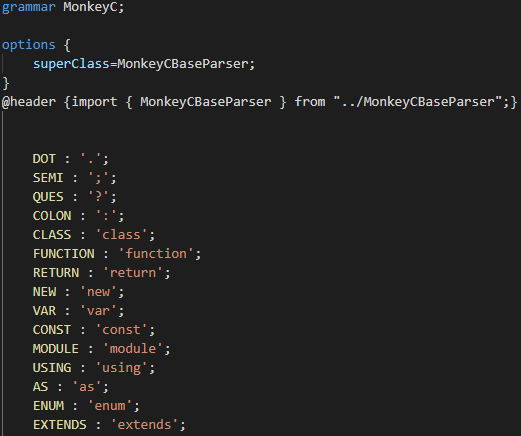
\includegraphics[scale=0.8]{images/grammar}
	\caption{ukázka hlavičky gramatiky MonkeyC.g4 pro popis jazyka}
	\label{img:grammar}
\end{figure}

\begin{figure}
	\centering
	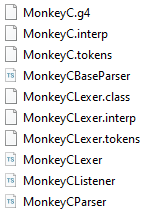
\includegraphics{images/generated_files}
	\\
	\caption{potřebné soubory vygenerované nástrojem ANTLR}
	\label{img:generated_files}
\end{figure}

\subsection{TestRig}
ANTLR poskytuje flexibilní testovací nástroj umístněný v runtime knihovně s názvem TestRig. TestRig dokáže poskytnout spoustu informací o tom, jak "recognizéry" (parser a lexer) zpracovávají InputStream ze vstupního souboru. TestRig je spouštěn z příkazového řádku pomocí aliasu \emph{grun}. Nabízí spoustu možností, jak zobrazit vygenerovaný syntaktický strom:
\begin{enumerate}
\item \textbf{-tree}: zobrazí syntaktický strom jako soubor do sebe zanořených pravidel gramatiky
\item \textbf{-tokens}: výstupem jsou tokeny, které parser vygeneroval ze vstupních dat
\item \textbf{-gui}: zobrazí syntaktický strom vizuálně v programu ParseTreeInspector, který je součástí ANTLR. Příklad zobrazení jednoduchého vstupu bez detekovaných chyb lze vidět na obrázku \ref{img:ParseTreeInspector}. Dále lze na obrázku vidět, jak jsou mezi sebou jednotlivé části stromu, tedy uzly, navzájem propojeny. Strom začíná kořenem, jenž je v gramatice pojmenován, jako "program". Takto je kořen pojmenován při každém parsování. 
\end{enumerate}

Podle mého názoru se jedná o užitečný nástroj, který uživateli poskytuje přehled o tom, zda parser rozpoznal vstupní data správně, případně kde parser detekovat rozpory z gramatikou. Při vývoji a testování rozšíření byl tento nástroj velmi kvalitním pomocníkem. Možností, které pro testování gramatik a parserů TestRig nabízí, je samozřejmě více, ale pro účely této práce byly použity hlavně tři výše uvedené. 

\begin{figure}
	\centering
	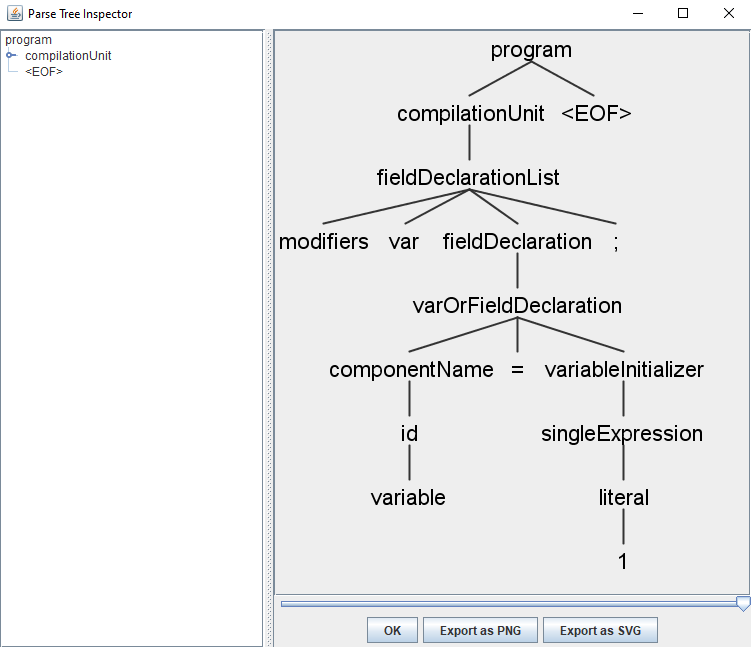
\includegraphics[scale=0.8]{images/ParseTreeInspector}
	\caption{"ParseTreeInspector" - vizuální podoba syntaktického stromu} 
	\label{img:ParseTreeInspector}
\end{figure}

\endinput